% Options for packages loaded elsewhere
\PassOptionsToPackage{unicode}{hyperref}
\PassOptionsToPackage{hyphens}{url}
%
\documentclass[
  ignorenonframetext,
]{beamer}
\usepackage{pgfpages}
\setbeamertemplate{caption}[numbered]
\setbeamertemplate{caption label separator}{: }
\setbeamercolor{caption name}{fg=normal text.fg}
\beamertemplatenavigationsymbolshorizontal
% Prevent slide breaks in the middle of a paragraph
\widowpenalties 1 10000
\raggedbottom
\setbeamertemplate{part page}{
  \centering
  \begin{beamercolorbox}[sep=16pt,center]{part title}
    \usebeamerfont{part title}\insertpart\par
  \end{beamercolorbox}
}
\setbeamertemplate{section page}{
  \centering
  \begin{beamercolorbox}[sep=12pt,center]{part title}
    \usebeamerfont{section title}\insertsection\par
  \end{beamercolorbox}
}
\setbeamertemplate{subsection page}{
  \centering
  \begin{beamercolorbox}[sep=8pt,center]{part title}
    \usebeamerfont{subsection title}\insertsubsection\par
  \end{beamercolorbox}
}
\AtBeginPart{
  \frame{\partpage}
}
\AtBeginSection{
  \ifbibliography
  \else
    \frame{\sectionpage}
  \fi
}
\AtBeginSubsection{
  \frame{\subsectionpage}
}

\usepackage{amsmath,amssymb}
\usepackage{iftex}
\ifPDFTeX
  \usepackage[T1]{fontenc}
  \usepackage[utf8]{inputenc}
  \usepackage{textcomp} % provide euro and other symbols
\else % if luatex or xetex
  \usepackage{unicode-math}
  \defaultfontfeatures{Scale=MatchLowercase}
  \defaultfontfeatures[\rmfamily]{Ligatures=TeX,Scale=1}
\fi
\usepackage{lmodern}
\usetheme[]{default}
\ifPDFTeX\else  
    % xetex/luatex font selection
\fi
% Use upquote if available, for straight quotes in verbatim environments
\IfFileExists{upquote.sty}{\usepackage{upquote}}{}
\IfFileExists{microtype.sty}{% use microtype if available
  \usepackage[]{microtype}
  \UseMicrotypeSet[protrusion]{basicmath} % disable protrusion for tt fonts
}{}
\makeatletter
\@ifundefined{KOMAClassName}{% if non-KOMA class
  \IfFileExists{parskip.sty}{%
    \usepackage{parskip}
  }{% else
    \setlength{\parindent}{0pt}
    \setlength{\parskip}{6pt plus 2pt minus 1pt}}
}{% if KOMA class
  \KOMAoptions{parskip=half}}
\makeatother
\usepackage{xcolor}
\newif\ifbibliography
\setlength{\emergencystretch}{3em} % prevent overfull lines
\setcounter{secnumdepth}{-\maxdimen} % remove section numbering


\providecommand{\tightlist}{%
  \setlength{\itemsep}{0pt}\setlength{\parskip}{0pt}}\usepackage{longtable,booktabs,array}
\usepackage{calc} % for calculating minipage widths
\usepackage{caption}
% Make caption package work with longtable
\makeatletter
\def\fnum@table{\tablename~\thetable}
\makeatother
\usepackage{graphicx}
\makeatletter
\def\maxwidth{\ifdim\Gin@nat@width>\linewidth\linewidth\else\Gin@nat@width\fi}
\def\maxheight{\ifdim\Gin@nat@height>\textheight\textheight\else\Gin@nat@height\fi}
\makeatother
% Scale images if necessary, so that they will not overflow the page
% margins by default, and it is still possible to overwrite the defaults
% using explicit options in \includegraphics[width, height, ...]{}
\setkeys{Gin}{width=\maxwidth,height=\maxheight,keepaspectratio}
% Set default figure placement to htbp
\makeatletter
\def\fps@figure{htbp}
\makeatother

\newcommand{\theHtable}{\thetable}
\usepackage{fontspec}
\usepackage{graphicx}
\usepackage{grffile}
\setkeys{Gin}{width=\textwidth,height=\textheight}
\makeatletter
\@ifpackageloaded{caption}{}{\usepackage{caption}}
\AtBeginDocument{%
\ifdefined\contentsname
  \renewcommand*\contentsname{Table of contents}
\else
  \newcommand\contentsname{Table of contents}
\fi
\ifdefined\listfigurename
  \renewcommand*\listfigurename{List of Figures}
\else
  \newcommand\listfigurename{List of Figures}
\fi
\ifdefined\listtablename
  \renewcommand*\listtablename{List of Tables}
\else
  \newcommand\listtablename{List of Tables}
\fi
\ifdefined\figurename
  \renewcommand*\figurename{Figure}
\else
  \newcommand\figurename{Figure}
\fi
\ifdefined\tablename
  \renewcommand*\tablename{Table}
\else
  \newcommand\tablename{Table}
\fi
}
\@ifpackageloaded{float}{}{\usepackage{float}}
\floatstyle{ruled}
\@ifundefined{c@chapter}{\newfloat{codelisting}{h}{lop}}{\newfloat{codelisting}{h}{lop}[chapter]}
\floatname{codelisting}{Listing}
\newcommand*\listoflistings{\listof{codelisting}{List of Listings}}
\makeatother
\makeatletter
\makeatother
\makeatletter
\@ifpackageloaded{caption}{}{\usepackage{caption}}
\@ifpackageloaded{subcaption}{}{\usepackage{subcaption}}
\makeatother

\ifLuaTeX
  \usepackage{selnolig}  % disable illegal ligatures
\fi
\usepackage{bookmark}

\IfFileExists{xurl.sty}{\usepackage{xurl}}{} % add URL line breaks if available
\urlstyle{same} % disable monospaced font for URLs
\hypersetup{
  pdftitle={Class 19},
  pdfauthor={Sarah E. Grabinski},
  hidelinks,
  pdfcreator={LaTeX via pandoc}}


\title{Class 19}
\subtitle{DATA1220-55, Fall 2024}
\author{Sarah E. Grabinski}
\date{2024-10-16}

\begin{document}
\frame{\titlepage}


\begin{frame}{Chapter 2 Objectives: Numerical Data}
\phantomsection\label{chapter-2-objectives-numerical-data}
\begin{itemize}
\item
  Describe the ``shape'' (i.e.~distribution) of numerical variables
\item
  Calculate means, medians, modes, variances, standard deviations, IQRs
\item
  Learn the appropriate use of summary statistics (i.e.~mean vs.~median)
\item
  Characterize the relationship between 2 numerical variables
\end{itemize}
\end{frame}

\begin{frame}{Chapter 2 Objectives: Categorical Data}
\phantomsection\label{chapter-2-objectives-categorical-data}
\begin{itemize}
\item
  Analyze contingency (e.g.~2x2) tables
\item
  Summarizing categorical variables with proportions
\item
  Comparison of numerical data between categorical groups
\end{itemize}
\end{frame}

\begin{frame}[fragile]{Chapter 2 Objectives: Visualizing Data}
\phantomsection\label{chapter-2-objectives-visualizing-data}
\begin{itemize}
\item
  Recognize common visualization techniques / plots

  \begin{itemize}
  \item
    Numerical: Dot plots, histograms, density plots, box plots, violin
    plots
  \item
    Categorical: bar plots, mosaic plots, tree map
  \end{itemize}
\item
  Build basic visualizations in \texttt{R} using \texttt{ggplot2}
\end{itemize}
\end{frame}

\begin{frame}{Distribution Checklist}
\phantomsection\label{distribution-checklist}
\begin{itemize}
\item
  Modality
\item
  Symmetry
\item
  Skew
\item
  Outliers
\item
  Summary Statistics
\end{itemize}
\end{frame}

\begin{frame}{Modality}
\phantomsection\label{modality}
How many ``peaks'' are there?

\begin{itemize}
\item
  \textbf{\emph{Unimodal}}: one peak
\item
  \textbf{\emph{Bimodal}}: two peaks
\item
  \textbf{\emph{Multimodal}}: many peaks
\item
  \textbf{\emph{Uniform}}: no clear peak, flat distribution
\end{itemize}
\end{frame}

\begin{frame}{Symmetry}
\phantomsection\label{symmetry}
Is there asymmetry in the distribution?

\begin{itemize}
\item
  \textbf{\emph{Symmetric}}: ``mirror image'', the distribution to the
  left of center looks like the distribution to the right of center
\item
  \textbf{\emph{Asymmetric}}: left half looks different than the right
  half
\end{itemize}
\end{frame}

\begin{frame}{Skew}
\phantomsection\label{skew}
If the distribution is asymmetric, is it because it's skewed?

\begin{itemize}
\item
  Does the distribution ``lean'' towards the left or the right?
\item
  Does the distribution have a long ``tail'' on one side but not the
  other?
\end{itemize}
\end{frame}

\begin{frame}[fragile]{Outliers}
\phantomsection\label{outliers}
Are there any unusual data points?

\begin{verbatim}
-   How extreme are the most extreme values?

-   Outliers are *rare*

-   When data points are unusual but not rare, they create *skew* or *modality*
\end{verbatim}
\end{frame}

\begin{frame}{Summary Statistics}
\phantomsection\label{summary-statistics}
Is the distribution normal or does it require robust statistics?

\begin{figure}[H]

{\centering 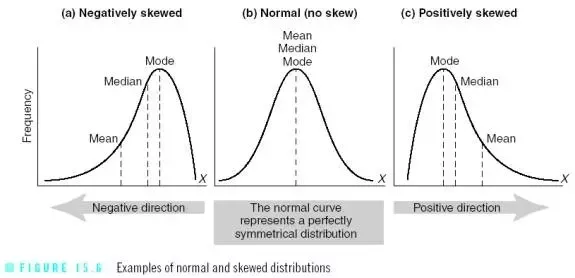
\includegraphics{class05/outlier_statistics.png}

}

\caption{The presence of outliers and/or skew in a numerical variable's
distribution affects how well summary statistics describe a
distribution's location.}

\end{figure}%
\end{frame}

\begin{frame}{Robust statistics}
\phantomsection\label{robust-statistics}
The \textbf{\emph{median}} and \textbf{\emph{interquartile range}} are
considered to be \textbf{\emph{robust statistics}} for the numerical
summary of data because they are less sensitive to \textbf{\emph{skew}}
and \textbf{\emph{outliers}} than the \textbf{\emph{mean}} and
\textbf{\emph{standard deviation}}.

\begin{figure}[H]

{\centering 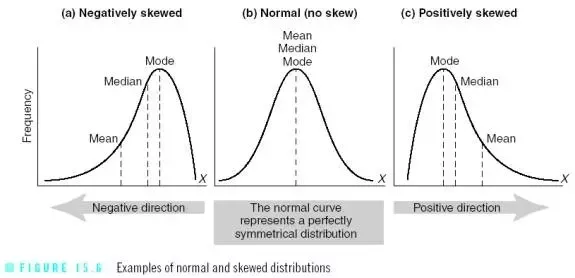
\includegraphics{class05/outlier_statistics.png}

}

\caption{The presence of outliers and/or skew in a numerical variable's
distribution affects how well summary statistics describe a
distribution's location.}

\end{figure}%
\end{frame}

\begin{frame}{5-Number Summary of Numerical Data}
\phantomsection\label{number-summary-of-numerical-data}
\begin{enumerate}
\item
  Minimum value or Q1 - 1.5 x Interquartile Region
\item
  1st quartile (Q1, 25th percentile)
\item
  Median (Q2, 50th percentile)
\item
  3rd quartile (Q3, 75th percentile)
\item
  Maximum value or Q3 + 1.5 x Interquartile Region
\end{enumerate}
\end{frame}

\begin{frame}{Choosing Summary Statistics for Numerical Data}
\phantomsection\label{choosing-summary-statistics-for-numerical-data}
\begin{itemize}
\item
  The \textbf{mean} and \textbf{standard deviation} are really only
  appropriate for a certain type of unimodal, symmetric distribution
  called the \textbf{normal distribution} and often misused
\item
  Most real world data will be best described by the \textbf{median} and
  \textbf{interquartile region} as part of a 5-number summary
\end{itemize}
\end{frame}

\begin{frame}{Anatomy of a Boxplot}
\phantomsection\label{anatomy-of-a-boxplot}
\begin{figure}[H]

{\centering 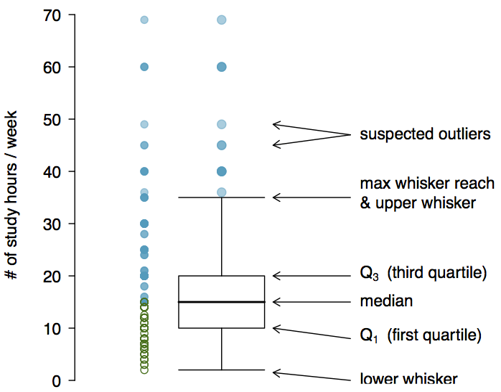
\includegraphics{class06/boxplot_anatomy.png}

}

\caption{A boxplot is a visual representation of a 5-number summary. The
``box'' represents the middle 50\% of the data, or the interquartile
range. The line inside the box indicates the median or 50th percentile.
The whiskers, the lines coming out from the box, extend 1.5 x IQR beyond
Q1 and Q3. Values larger or smaller than that range are classified as
outliers and appear as points.}

\end{figure}%
\end{frame}

\begin{frame}{Boxplot whiskers and outliers}
\phantomsection\label{boxplot-whiskers-and-outliers}
\begin{itemize}
\item
  The \textbf{\emph{whiskers}} of a boxplot (the lines extending out
  from the box) are 1.5 times the \textbf{\emph{interquartile region}}
  long

  \begin{itemize}
  \item
    Min whisker: Q1 - 1.5 x IQR
  \item
    Max whisker: Q3 + 1.5 x IQR
  \end{itemize}
\item
  If a point is outside this range, it is considered to be a potential
  \textbf{\emph{outlier}}
\end{itemize}
\end{frame}

\begin{frame}{Calculating Proportions by row}
\phantomsection\label{calculating-proportions-by-row}
\begin{figure}[H]

{\centering 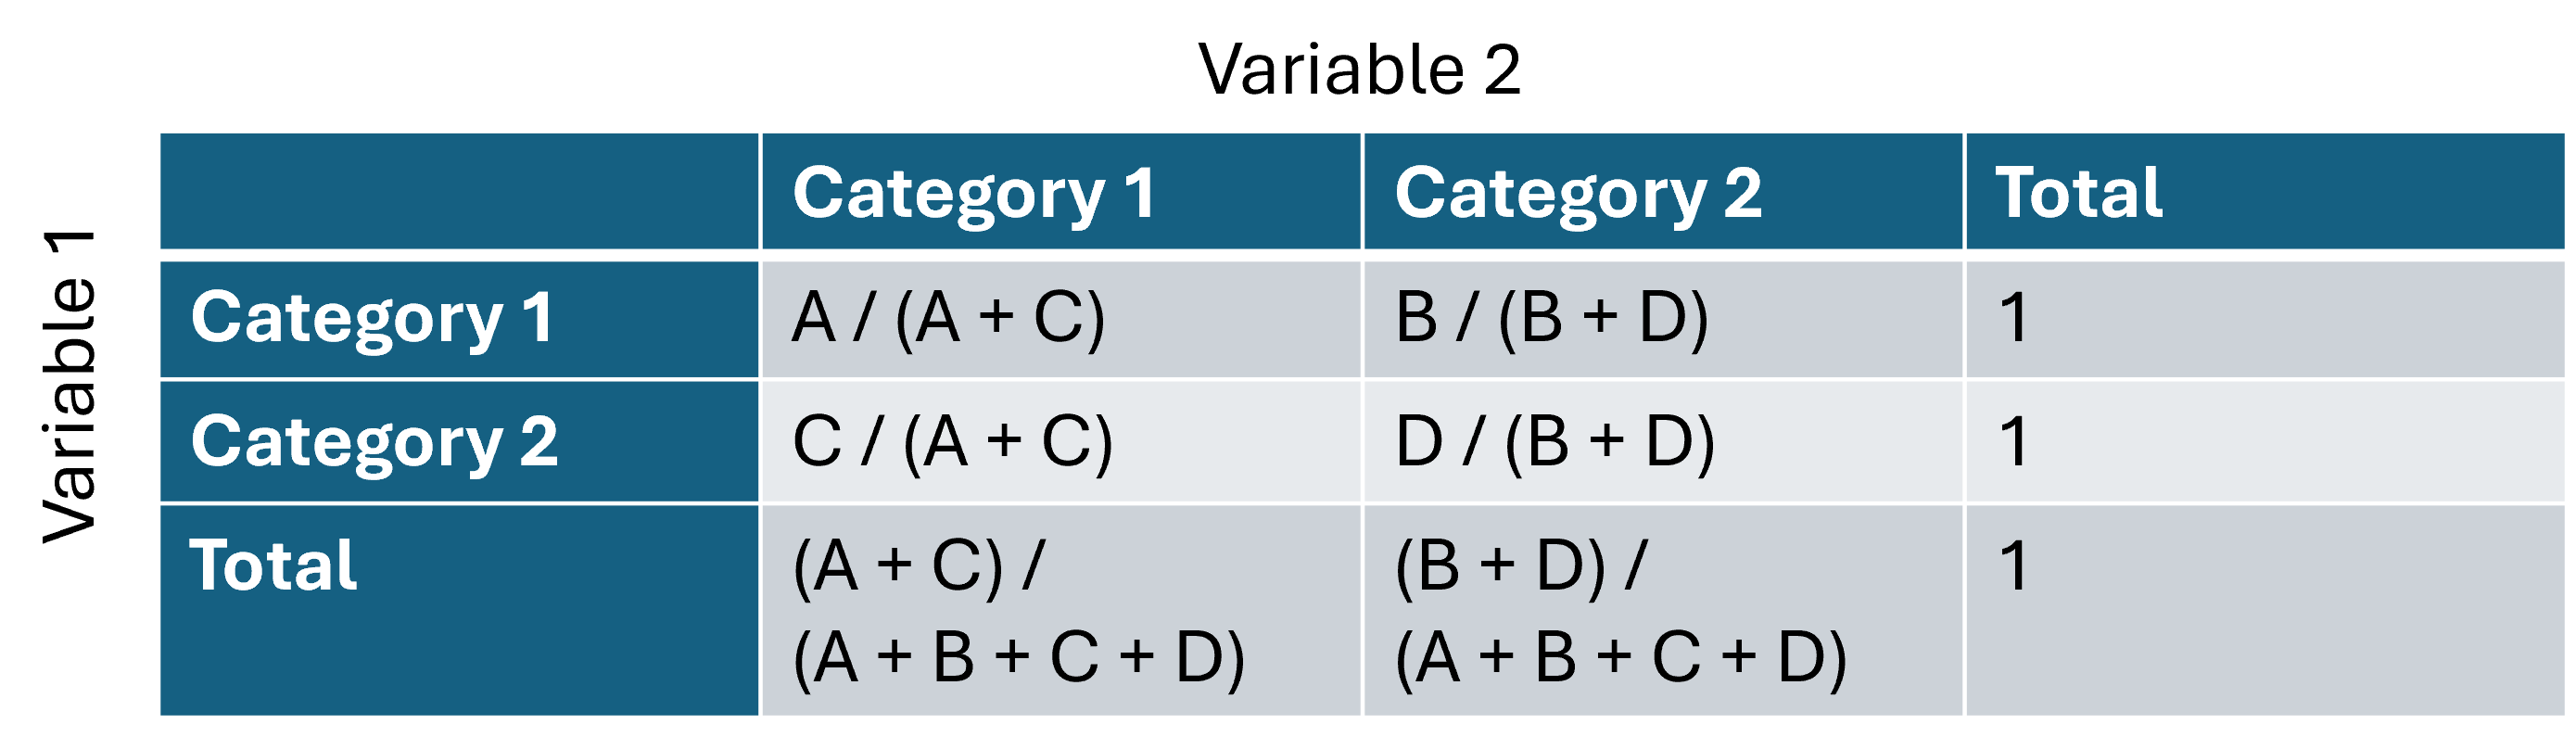
\includegraphics{class07/contingency-table-row-proportions.png}

}

\caption{The row totals are all 1, which is the maximum value of a
proportion. This indicates that the denominator for the proportions is
the row total for each cell.}

\end{figure}%
\end{frame}

\begin{frame}{Calculating Proportions by Column}
\phantomsection\label{calculating-proportions-by-column}
\begin{figure}[H]

{\centering 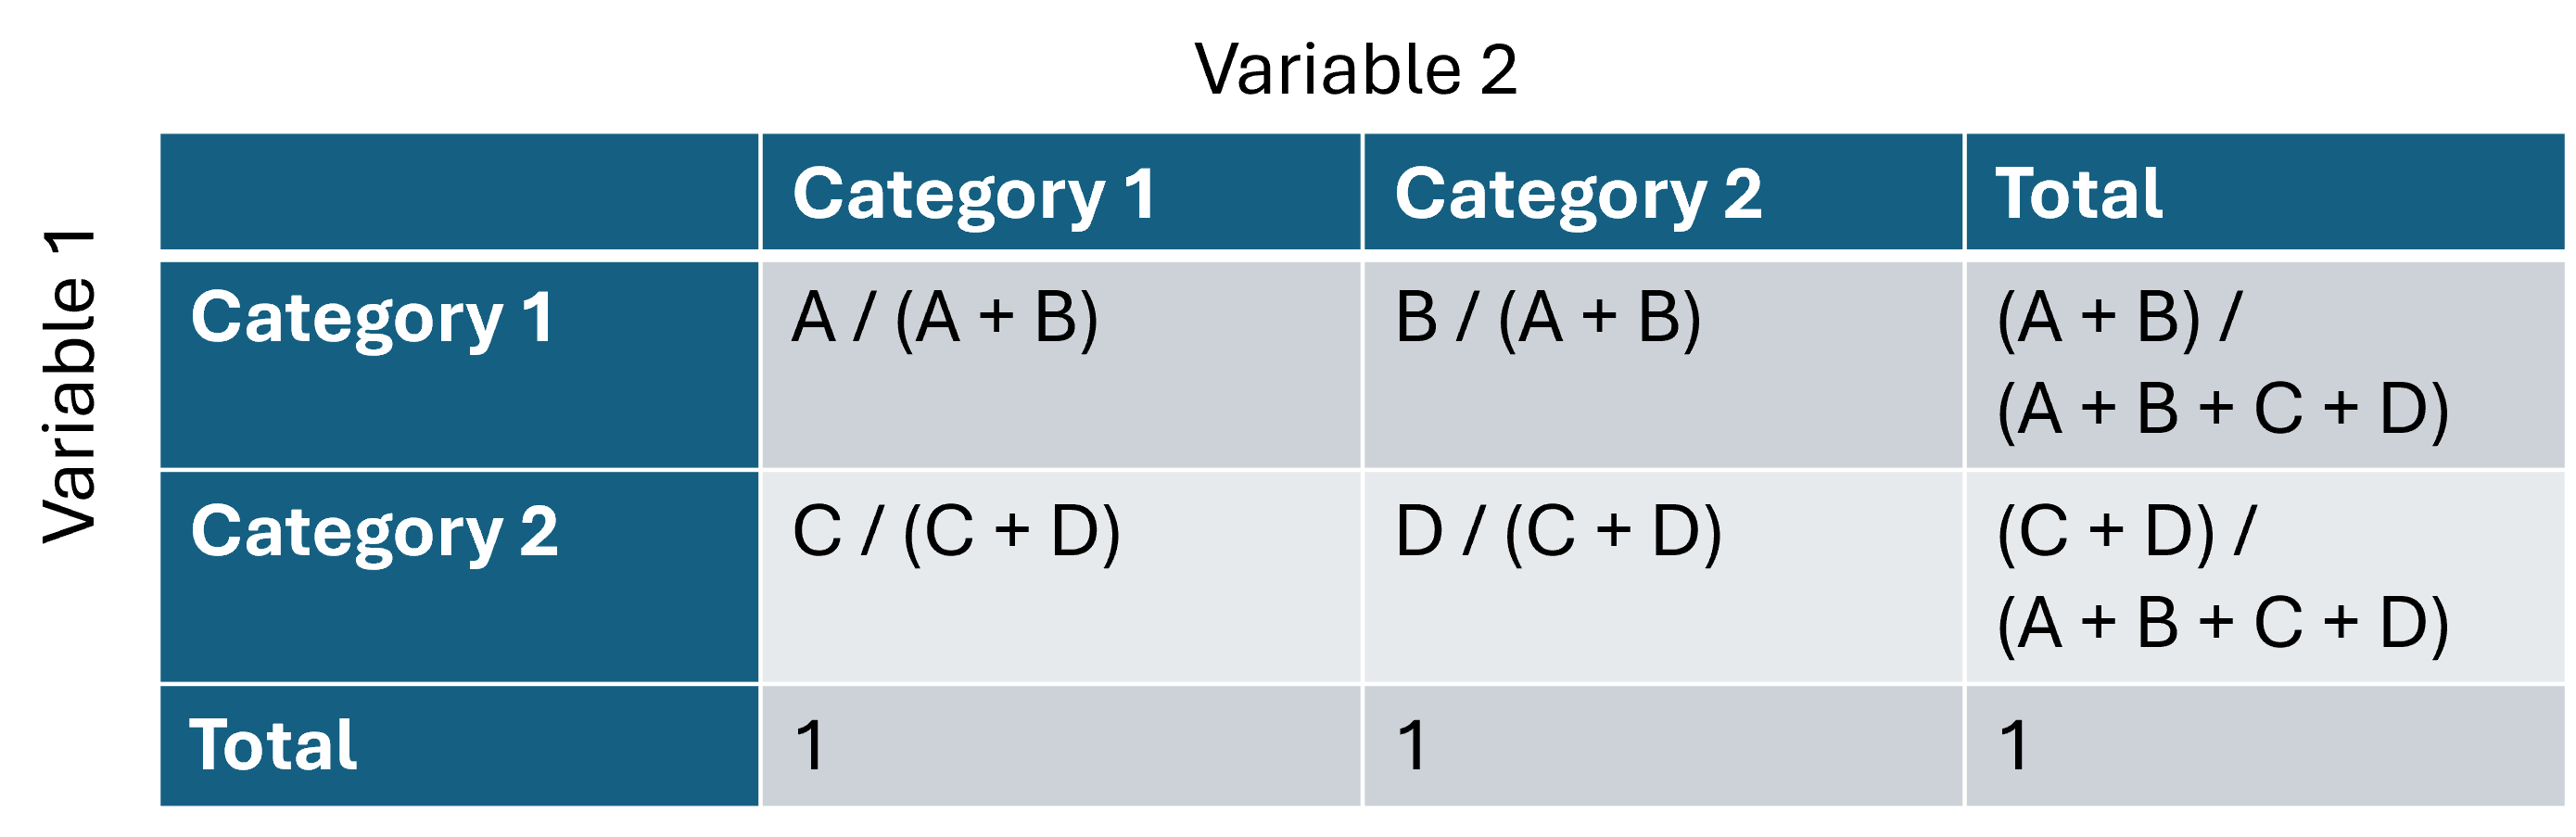
\includegraphics{class07/contingency-table-col-proportions.png}

}

\caption{The column totals are all 1, which is the maximum value of a
proportion. This indicates that the denominator for the proportions is
the column total for each cell.}

\end{figure}%
\end{frame}




\end{document}
